% !TEX root = master.tex
\subsection{Extracting 1D Profiles}
We extract two 1-dimensional profiles for each image. In our implementation, wedges drawn along each direction of the major axis centred by fitted isophote ellipses and the median counts are calculated along the axis at regular intervals (with central counts being determined by interpolation). The profile is terminated when the counts become consistently lower than the sky value given by SDSS/MegaCam pipeline. This results in four 1D profiles for each galaxy with varying sizes of regions where the sky becomes dominant. 

\subsection{Sky Subtraction}
\subsubsection{The effects of sky}
The night sky is never completely dark and in the \iband it has a brightness of $19.9$ mag $\rm{arcsec}^{-2}$ \citep{binney_galactic_1998}. Indeed, proficient sky subtraction is required for the acquisition of accurate surface brightness profiles at low brightness. If the sky background is underestimated, the sky will contribute to the profile at large galactic radius and flatten off the profile if sufficiently extended. If the background is overestimated, light from the galaxy is subtracted also, plunging it towards zero at some finite radius. 

\begin{figure}[h]
	\centering
	\makebox[0.9\columnwidth]{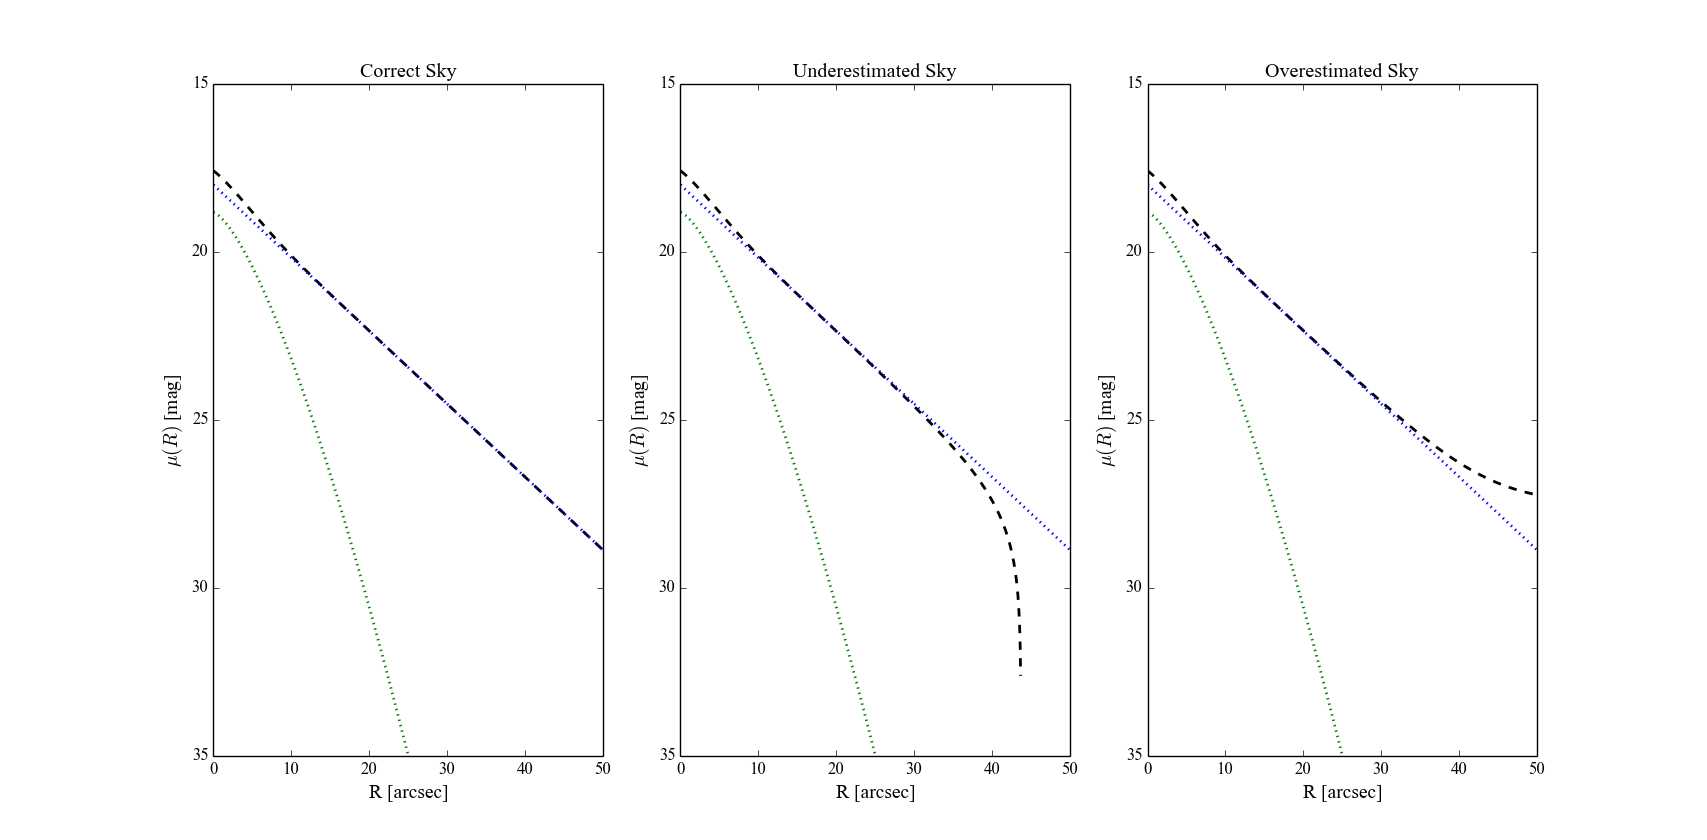
\includegraphics[width=1.5\textwidth]{figs/sky_examples.png}}
	\caption{\footnotesize{The effect of an error in the sky of $\pm 5$ counts}}
	\label{fig: effects of sky}
\end{figure}
There are, however, other errors that contribute to the overall corruption of the image besides sky estimation. Due to the limitations of optical devices and CCDs, there may be a gradient across an image frame to due to CCD bias or inhomogeneous illumination \citep{olsen_radiometric_2010}. Joining frames together, or `splicing' exacerbates this effect since different exposures will have different sky backgrounds. The raw data is already corrected for this by SDSS and MegaCam in flat-fielding corrections, but the correction is not perfect and may result in unwanted artefacts or gradients across the image. SDSS operates in drift scan mode \citep{abazajian_seventh_2009} and so does not suffer as much from the effects of flat-fielding since any bias or aberration is averaged out.

\subsubsection{Finding the Sky}
Accurate background estimates are essential in characterising outer profiles. While both cameras give their own estimated sky fluxes and the extraction of 1D profiles yields a additional estimate, background can vary within images -and between major axis profiles- due to flat-fielding errors \citep{bijaoui_sky_1980}. 

To find the radial position at which the sky starts to dominate, the profile is divided into chunks of three data points. For each chunk, the local mean and standard deviation are calculated. This is essentially finding the local value of intensity. We define the point at which the sky starts to dominate as the point where $\bar{I}_{i+1} > \bar{I}_i + \sigma_i$, where $\bar{I}_i$ is the local mean intensity and $\sigma_i$ is the standard deviation at point $i$. We initiate this search from the end of the profile. The effects of local minima and maxima due to stars and noise are also taken into account by considering the next two local means instead of just one (i.e. $\bar{I}_{i+2}$).

\begin{figure}[h]
	\centering
	\makebox[0.9\columnwidth]{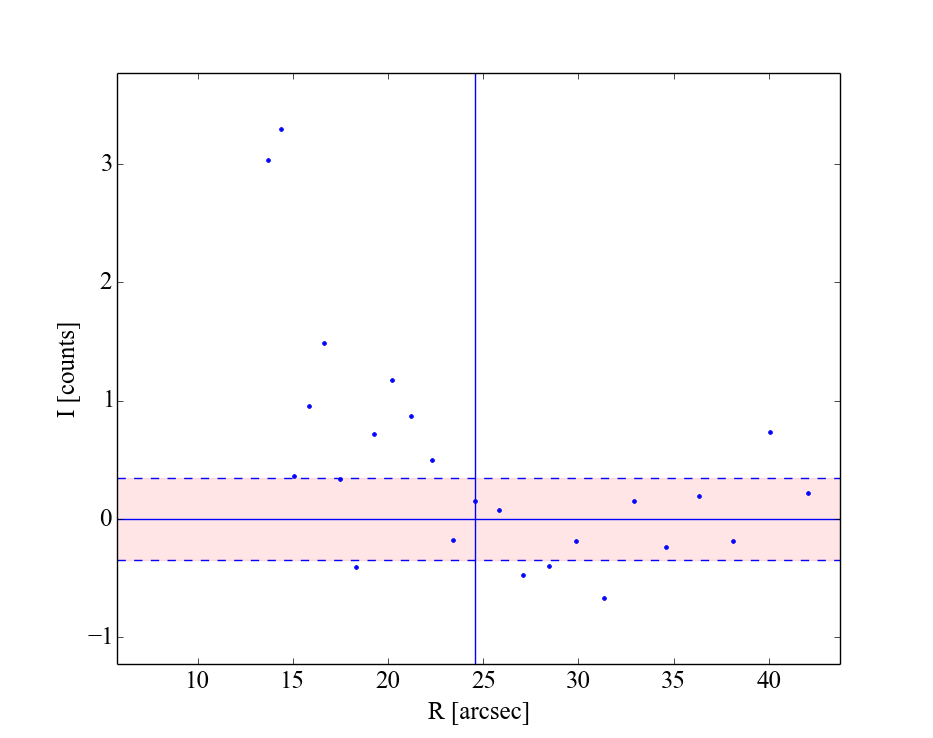
\includegraphics[width=0.6\textwidth]{figs/sky_finder.png}}
	\caption{\footnotesize{Area of the profile from 1237667324334506284 (MegaCam axis 1) with the sky uncertainty shown in red and the cut off point as the vertical straight line}}
\end{figure}

The mode is the best estimate for the sky value since it is the peak of the brightness frequency distribution \citep{bijaoui_sky_1980}. Therefore, we use a $3\sigma$-clipped, synthetic mode to estimate the sky values.

The value for sky uncertainty is calculated by first `clipping' the sky dominated area so that values that lie further than $3\sigma$ away from the mean sky value are removed. We use a similar synthetic mode to \citet{peng_detailed_2010} of $3(\rm{median}) - 2(\rm{mean})$ to calculate sky brightness along with its standard deviation for the sky uncertainty.

We define the critical surface brightness $\mu_{crit}$ as the surface brightness up to which the profile is considered reliable. $\mu_{crit}$ is placed where we calculate the difference between under and over subtracted profiles (i.e. $\pm 1 \sigma_{sky}$) to be 0.2 mag. This is a more useful measurement of sky than a $\pm 3 \sigma$ since it shows us where the actual profile starts to be affected.

\subsection{Bulge-Disc Decomposition}
\sersic parameters for each profile are determined by bulge-disc decomposition. We use the Levenberg-Marquardt non-linear least squares regression algorithm (LMA) to minimise chi-squared and fit the profile to the desired model. Reduced chi-squared is used as a goodness-of-fit measure.
\begin{equation}
	\chi^{2}_{\nu} = \frac{1}{N-n-1} \sum_{i} \frac{[y_i - f(x_i)]^2}{w_i^2},
\end{equation}
where $\chi_{\nu}^2$ is the reduced chi-squared goodness-of-fit measure, $N$ is the number of data points, $n$ is the number of free parameters, $y_i$ are the data points, $f(x_i)$ are the associated model points and $w_i$ are the associated weightings for each point \citep{marquardt_algorithm_1963}. A reduced chi-squared of $\chi_{\nu}^2 \approx 1$ describes an accurate fit, $\chi_{\nu}^2<1$ describes overestimated errors and $\chi_{\nu}^2>1$ is degenerate in describing both underestimated errors or an incorrect model. This is by far the most tested and reliable fitting method \citep{lawson_solving_1995} and was implemented in the high-level language Python with Scipy \citep{oliphant_python_2007}. 

We use an exponential disk + \sersic $R^{1/n}$ bulge model used in \citet{allen_millennium_2006} as bulges cannot all be described by $R^{1/4}$ \citep{simard_catalog_2011}. Fitting a model with six parameters is challenging to accomplish in one fell swoop since there is more parameter space to explore and so the likelihood of being trapped in a local minima -and not a global minima- increases. Therefore, we employ an iterative method similar to that found in \citet{weinzirl_bulge_2009} as follows:

\begin{enumerate}
	\item \sersic fit: \\
	A \sersic bulge (free $n_B$) is fit to the profile with a radial surface brightness of:
	\begin{equation}
		I(R) = I_{e} \rm{exp}\left\{-b_{n}\left[\left(\frac{R}{R_{e}}\right)^{1/n} - 1\right]\right\},
	\end{equation}
	where we use the definitions given earlier.	LMA converges quickly to a solution for a single \sersic roughly independent of initial parameter guesses. 

	\item Bulge+disk fit: \\
	The \sersic bulge is duplicated and has its \sersic index $n$ set to unity. The model now reads:
	\begin{equation}
		I(R) = I_0 \rm{exp}\left\{-\frac{R}{h}\right\} + I_{e} \rm{exp}\left\{-b_{n}\left[\left(\frac{R}{R_{e}}\right)^{1/n} - 1\right]\right\},
	\end{equation}
	where we now use the disc scale length $h=R_{e,disc}/1.678$ and central intensity $I_0=I_{e,disc}e^{-1.678}$ instead of $R_{e,disc}$ and $I_{e,disc}$ in order to distinguish concisely between bulge and disc parameters. 
\end{enumerate}

Fitting the usual assortment of effective magnitudes, effective radii and \sersic indices will sometimes result in an Allen Type-4 `inverted' profiles where the bulge dominates at large radii and the disk dominates at the centre \citep{allen_millennium_2006}. 

	Since we have already removed the sky and specified that we reject galaxies whose bulge dominates at large radii, we can assume that these solutions are likely the result of LMA attempting to fit a truncation or some other object such as a foreground star. To avoid these unreal solutions, the bulge+disk system is fit using effective radii difference and bulge-disk ratios (henceforth known as $\Delta R_e$ and $B/D$) instead of the parameters themselves. Limits are placed upon them such that $B/D < 1$ and $\Delta R_e = 1.678 h / R_e > 1$, to only permit disk dominated solutions. The bulge to disc ratio is

	\begin{equation}
		\frac{B}{D} = \frac{n \Gamma(2n)}{b^{2n}}\left(\frac{R_e}{h}\right)^{2} \left(\frac{I_e}{I_0}\right),
	\end{equation}
	where $b = b_{n,bulge}$.

Weights for use in LMA are computed in raw photon counts on a per pixel basis. The total error in intensity for each point is given by 
\begin{equation}
	\alpha = \frac{1}{s_{pix}^2}\sqrt{\alpha_I^2 + \alpha_{extraction}^2 + \alpha_{sky}^2},
\end{equation}

where $s_{pix}$ is the pixel scale, $\alpha_{extraction}$ is the error in forming a 1D profile along the major axis, $\alpha_{sky}$ is the sky uncertainty and $\alpha_I$ is the error in counts given by 
\begin{equation}
	\frac{\sqrt{I_{phot}G}}{G},
\end{equation}
where $I_{phot}$ is the raw photon count and $G$ is the CCD gain.

\subsection{Truncation Detection}
Fitting a galaxy with an un-truncated model, as above, is helpful to quantify the bulge size. It even gives some measure of truncation type through its residuals. 

To quantify a truncated surface brightness profile, three bulge parameters; two sets of scale lengths and central magnitudes; and a break radius are required. We do not fit a truncated model straight to the whole surface brightness profile as this is yet more unstable than the five parameter bulge-disc model due to the additional four parameters needed. We use a method similar to that of \citet{pohlen_structure_2006} whereby we instead, derive the break radius and then fit the truncated disk to the disk dominated area.

We define a disk dominated region where the disk is not more than 0.2 mag away from the total surface brightness and is not smaller than $\mu_{crit}$. This avoids noise from both the sky and the bulge.

\begin{figure}[h]
	\centering
	\makebox[0.5\columnwidth]{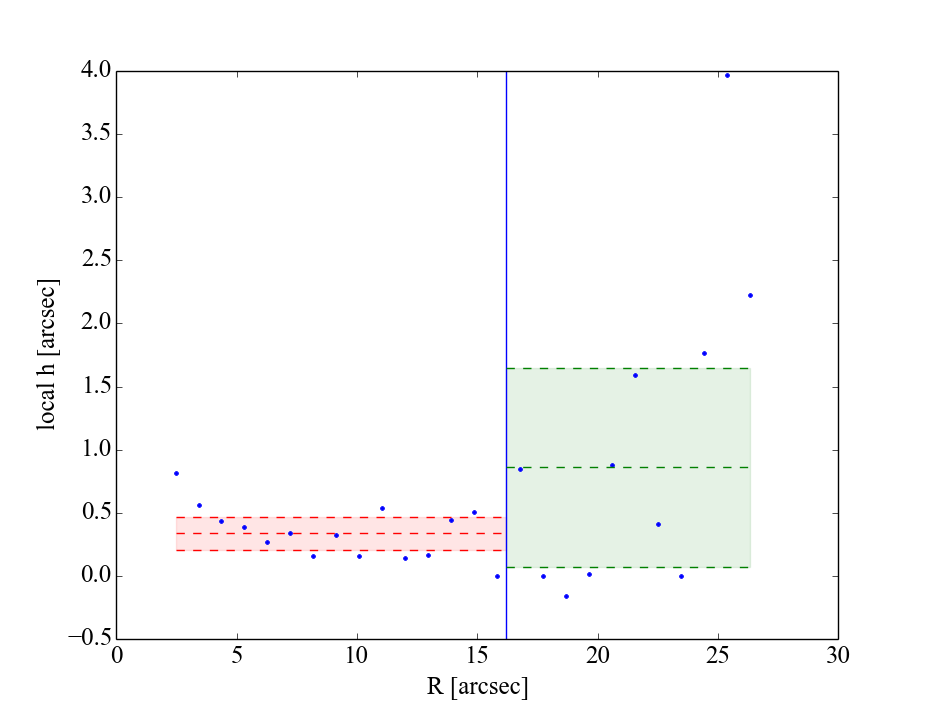
\includegraphics[width=0.8\textwidth]{figs/trunc_finder.png}}
	\caption{\footnotesize{Truncation break radius derivation for 1237667324334506284 (MegaCam axis 2). Standard deviations for each side are shown.}}
\end{figure}

The new disk profile is first smoothed using an unweighted B-spline function \citep{dierckx_curve_1975} of order 3. Then a median-filter is used to remove the last of extreme values with a smoothing length of 10\% of the length of the region.
The profile is then broken into overlapping chunks of three data points, to which a straight line is fitted. This results in an approximated derivative of the profile and estimate of the local scale length $h_{loc}$ at each point. 

Since the transition from scale lengths at the break radius has been found to be frequently smooth \citep{erwin_outer_2008,pohlen_stellar_2004,maltby_anti-truncated_2011}, we assume that there are now two regions of constant scale length joined by a transition region. 

We define the boundaries of the transition region as the point where the local scale length - starting from the break radius - reaches a value of $1\sigma$ away from the inner and outer means. These boundaries provide a measure for break radius uncertainty. 

We then proceed to fit a straight line to the magnitudes of both the inner and outer disk regions. We do not use the intensity counts because the outer disk is usually plagued with negative values and it is less computationally intensive. Due to the fact that the break region may be large, we do not restrict ourselves to not fitting inside it.

We fit the truncated disk using break radius, outer scale length, outer central surface brightness and scale length difference:
\begin{equation}
	\mu_{outer} = \mu_{0, outer} + 1.068 \frac{R}{h_{outer}}
\end{equation}
\begin{equation}
	\mu_{inner} = \mu_{0, outer} - \Delta\mu + 1.068R\left(\frac{1}{h_{outer}} + \Delta h\right)
\end{equation}
\begin{equation}
	\Delta \mu = 1.086R_{brk} \Delta h  = \mu_{outer} - \mu_{inner}
\end{equation}
\begin{equation}
	\Delta h = \frac{1}{h_{inner}} - \frac{1}{h_{outer}},
\end{equation}
where $\mu_{inner}$ is the surface brightness of the inner disk, $\mu_{0}$ is the central surface brightness, $h$ is the scale length and $R_{brk}$ is the break radius, which was restricted between the boundaries established during detection.

Classification of three or more such breaks is not uncommon in other works \citep{pohlen_structure_2006,gutierrez_outer_2011} but does lead to complications when trying to find the means around each break radius. In our investigation, it is assumed that there are no more than two break radii and this works well for the majority of cases. 

\subsection{Parameter Uncertainties}
The uncertainties of LMA can be computed from the covariance matrix of a fit \citep{hughes_measurements_2010}, but we implement a bootstrapping resampling procedure to estimate the errors on each fit parameter. 

We resample our data points, with replacement, and fit 1000 times to get a distribution for each parameter. The standard deviations and means are then calculated from this distribution.

In addition to the errors due to sampling and fitting (measured by bootstrapping), we calculate the error due to sky uncertainty. The profile is adjusted to 200 values within the sky uncertainty and the truncation algorithm is run for each of the new sky brightnesses We use these parameters as confidence intervals for the truncated disk since the limiting factor for characterising the outer disk is the sky level.